\documentclass{beamertmd}
\usetheme{tmd}

\usepackage{graphicx}

\title{MATLAB Toolbox for WBM}
\author{Nidish Narayanaa Balaji}
\begin{document}
\maketitle

\begin{frame}{Example: Jointed EB-Beam}  
  \begin{columns}
    \begin{column}{.5\textwidth}
      \begin{figure}
        \centering
        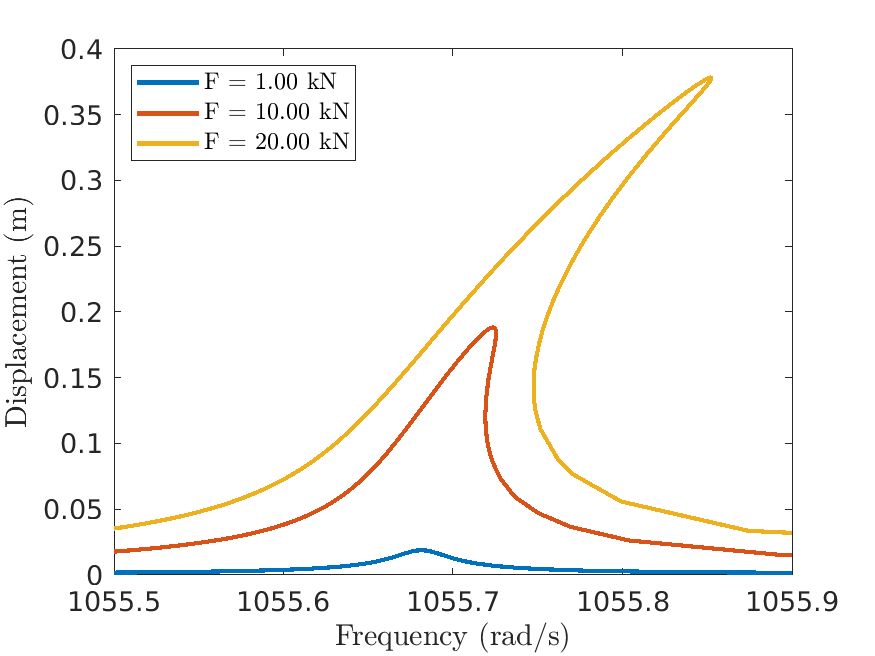
\includegraphics[width=\linewidth]{FIGS/fresp_EBBEAMJ}
        \caption{Forced Response}
      \end{figure}
    \end{column}

    \begin{column}{.5\textwidth}
      \begin{figure}
        \centering
        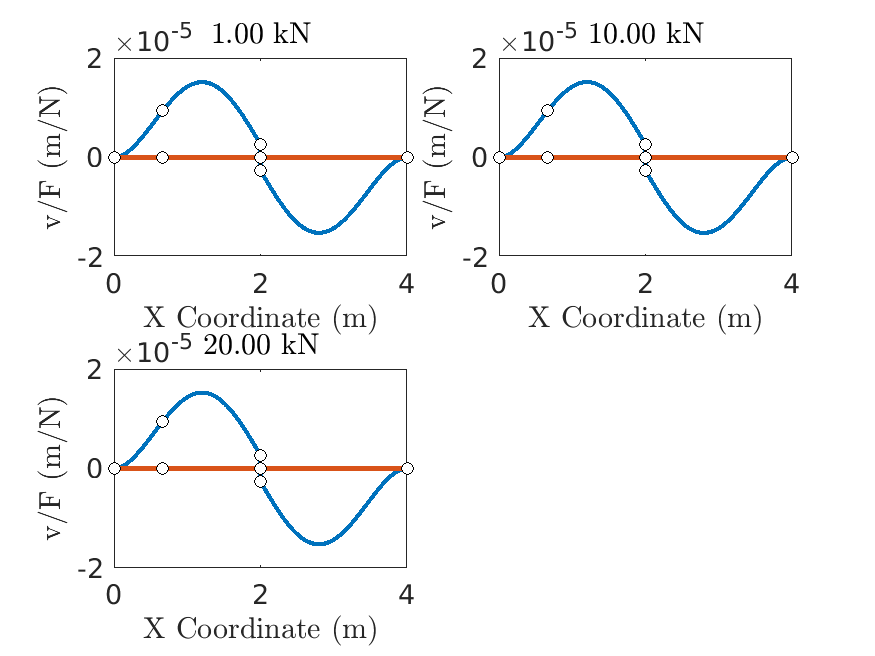
\includegraphics[width=\linewidth]{FIGS/dshape_EBBEAMJ}
        \caption{Deflection Shape}
      \end{figure}
    \end{column}
  \end{columns}
\end{frame}

\begin{frame}[allowframebreaks]
  \frametitle{Toolbox Plan}
  \begin{figure}
    \centering
    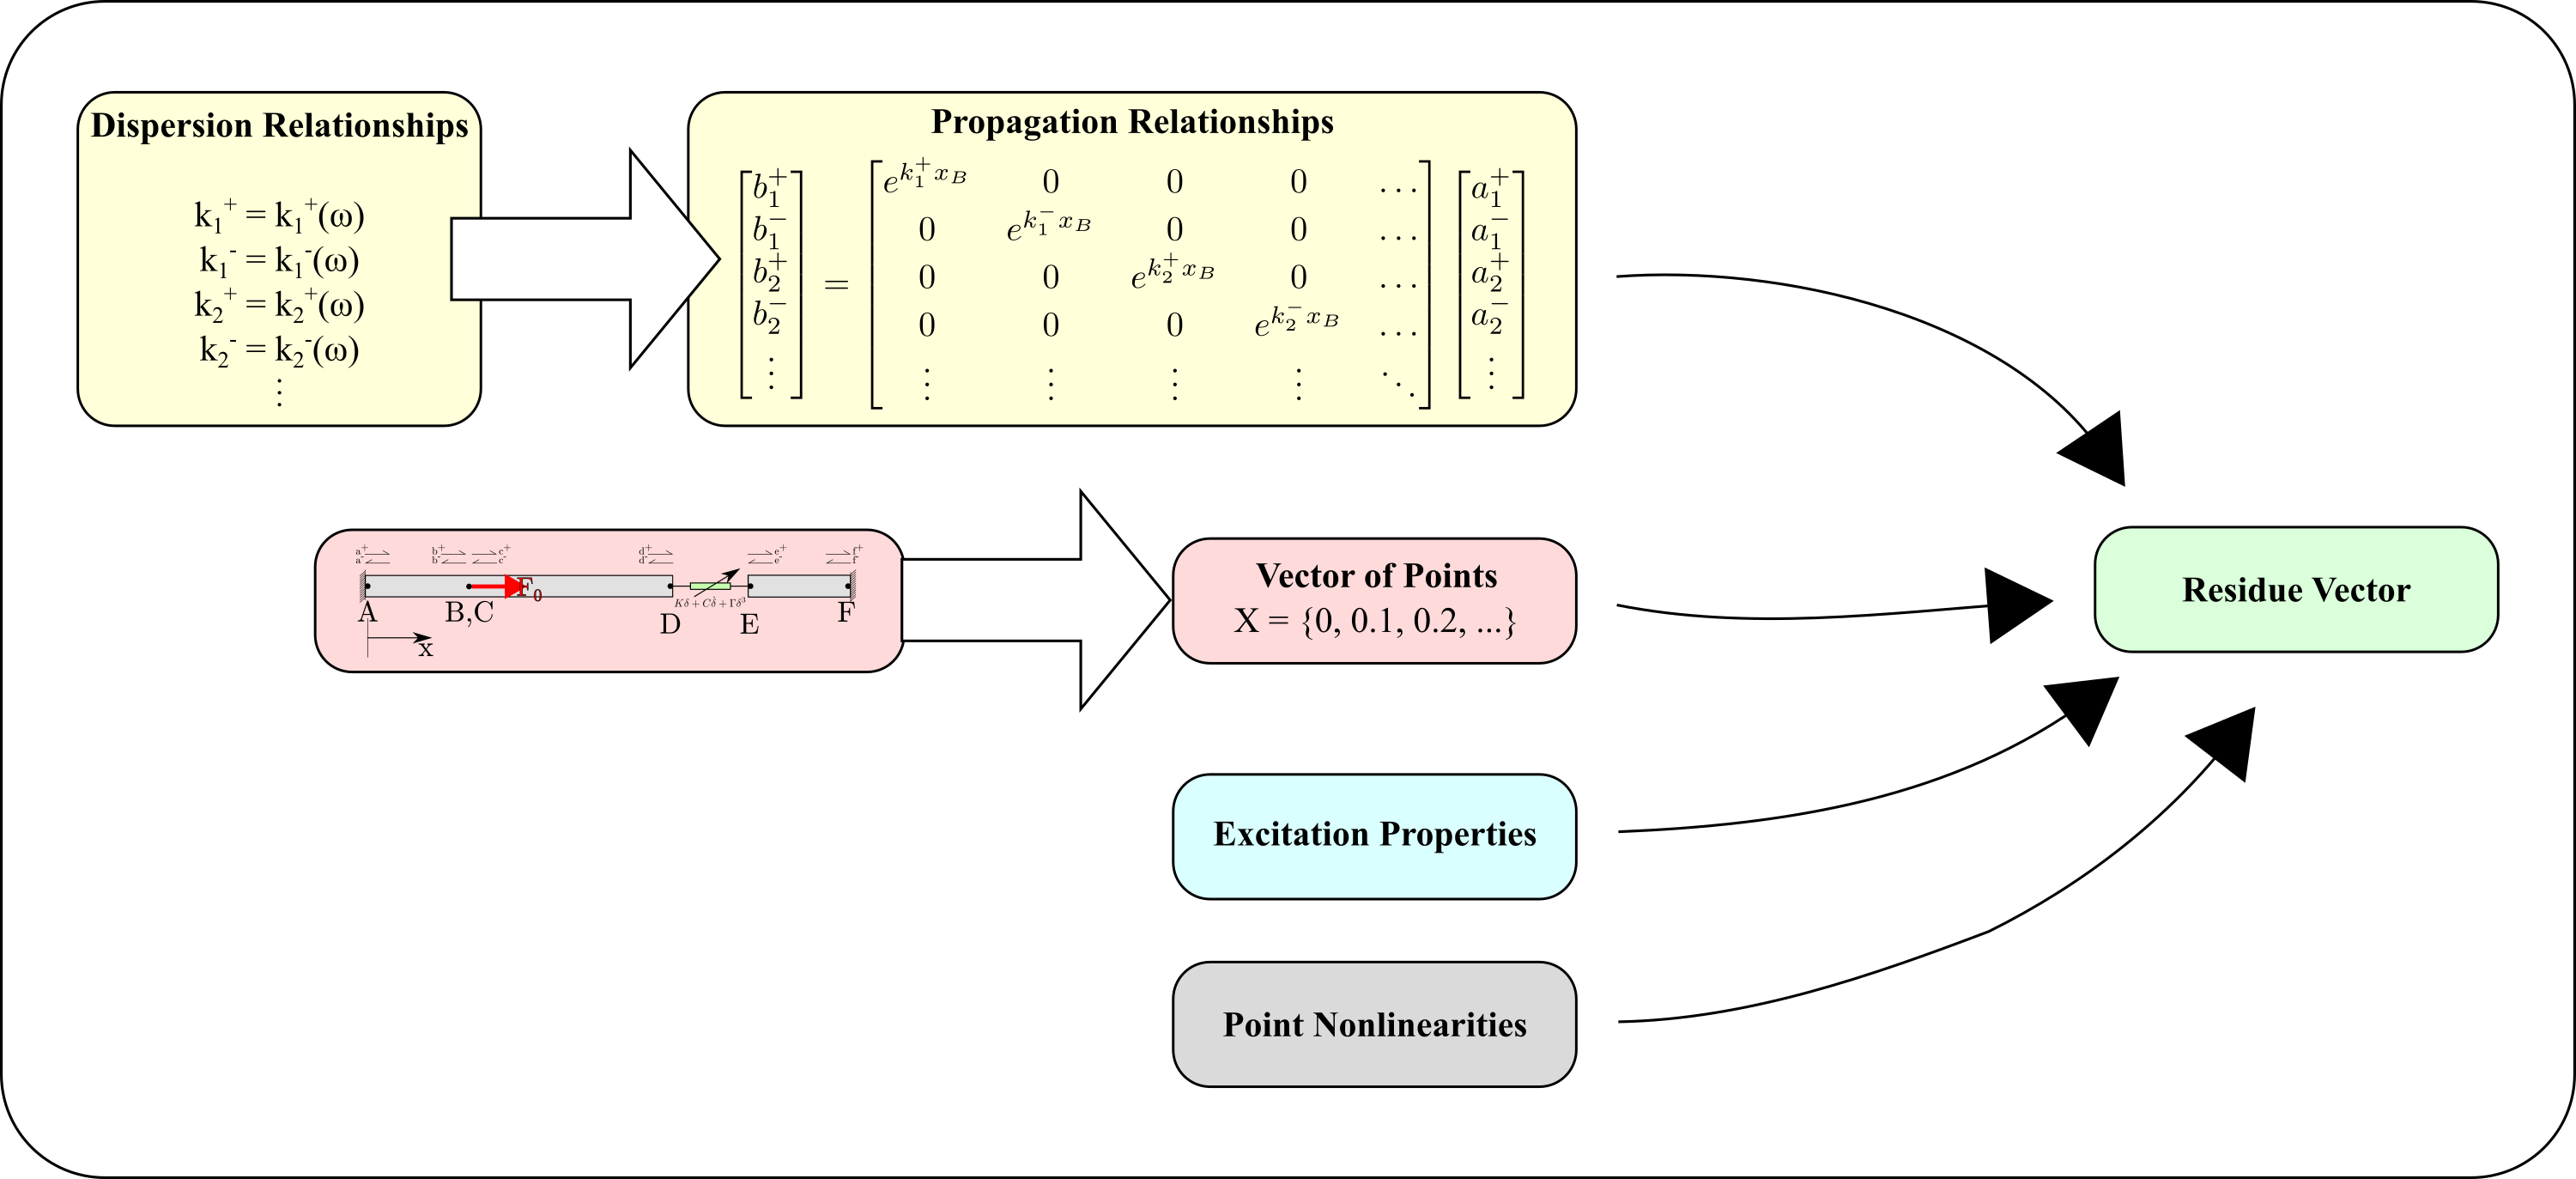
\includegraphics[width=\linewidth]{FIGS/rep1_SWPlan}
  \end{figure}
  \pagebreak
  \begin{itemize}
  \item Allows user to input arbitrary dispersion relationships for
    the different ``pieces'' in the model.
  \item Have implemented an \textbf{efficient symbolic
      differentiation} for all the expressions, making the Jacobian
    evaluations reliably fast, while ensuring the user doesn't need to
    type these in.
  \item Have validated the code for the bar examples in our paper as
    well as a jointed Euler-Bernoulli Beam example. 
  \item \textbf{Muli-Harmonic}, allows for PWE-type harmonic balance
    (\& stability), EPMC, etc.
  \end{itemize}
  \pagebreak
  \textbf{Need to do:}
  \begin{itemize}
  \item Only binary joints are implemented. Higher order joints can be
    implemented, but has to be done. 
  \item Schur complement based decomposition to make the nonlinear
    solves much more efficient. 
  \item Implementing constitutive relationships for 3D frame joints
    (direction cosines are available for each ``piece''). 
  \item Curved members?
  \end{itemize}
\end{frame}
\end{document}
%%% Local Variables:
%%% mode: latex
%%% TeX-master: t
%%% End:
